% !TeX program = lualatex

\documentclass[aspectratio=169,xcolor={dvipsnames}
,hide notes
%,show only notes
%,show notes on second screen=right
]{beamer}
\usetheme[background=light, numbering=fraction]{metropolis}
\usepackage{appendixnumberbeamer}

%\usepackage[T1]{fontenc}

\usepackage[labelfont=bf,textfont={it}]{caption}
\usepackage{subcaption}
\captionsetup[figure]{justification=centering}
\captionsetup[subfigure]{justification=centering}

\usepackage{tikz}
\usetikzlibrary{arrows.meta, calc, fit, positioning}

%\usepackage{fontspec}
%\setsansfont{Fira Sans Mono}

\usepackage[binary-units]{siunitx}
\sisetup{detect-all, range-phrase=--, range-units=single}

\usepackage[UKenglish]{babel}
\usepackage{csquotes}

\usepackage{amssymb}

\usepackage{lipsum}
\usepackage[basic]{complexity}
\usepackage[super,negative]{nth}

\usepackage{booktabs}

%bib
\usepackage[maxnames=3,maxbibnames=99,mincrossrefs=5,sortcites
,backend=bibtex
,style=authortitle
]{biblatex}
\addbibresource{../paper/papers-off.bib}
\addbibresource{../paper/confs-off.bib}
\addbibresource{../paper/books-off.bib}
\addbibresource{../paper/rfc.bib}
\addbibresource{../paper/misc.bib}

\makeatletter
\DeclareRobustCommand{\rvdots}{%
	\vbox{
		\baselineskip4\p@\lineskiplimit\z@
		\kern-\p@
		\hbox{.}\hbox{.}\hbox{.}
}}
\makeatother

% official colours
\definecolor{uofguniversityblue}{rgb}{0, 0.219608, 0.396078}

\definecolor{uofgheather}{rgb}{0.356863, 0.32549, 0.490196}
\definecolor{uofgaquamarine}{rgb}{0.603922, 0.72549, 0.678431}
\definecolor{uofgslate}{rgb}{0.309804, 0.34902, 0.380392}
\definecolor{uofgrose}{rgb}{0.823529, 0.470588, 0.709804}
\definecolor{uofgmocha}{rgb}{0.709804, 0.564706, 0.47451}

\definecolor{uofglawn}{rgb}{0.517647, 0.741176, 0}
\definecolor{uofgcobalt}{rgb}{0, 0.615686, 0.92549}
\definecolor{uofgturquoise}{rgb}{0, 0.709804, 0.819608}
\definecolor{uofgsunshine}{rgb}{1.0, 0.862745, 0.211765}
\definecolor{uofgpumpkin}{rgb}{1.0, 0.72549, 0.282353}
\definecolor{uofgthistle}{rgb}{0.584314, 0.070588, 0.447059}
\definecolor{uofgpillarbox}{rgb}{0.701961, 0.047059, 0}
\definecolor{uofglavendar}{rgb}{0.356863, 0.301961, 0.580392}

\definecolor{uofgsandstone}{rgb}{0.321569, 0.278431, 0.231373}
\definecolor{uofgforest}{rgb}{0, 0.317647, 0.2}
\definecolor{uofgburgundy}{rgb}{0.490196, 0.133333, 0.223529}
\definecolor{uofgrust}{rgb}{0.603922, 0.227451, 0.023529}

%picky abt et al.
\usepackage{xpatch}

\xpatchbibmacro{name:andothers}{%
	\bibstring{andothers}%
}{%
	\bibstring[\emph]{andothers}%
}{}{}

%opening!

\usepackage{cleveref}
\newcommand{\crefrangeconjunction}{--}

\usepackage{fontawesome}

%-------------------------------------%
%-------------------------------------%

\title{Improving Direct-Control Reinforcement Learning for Network Intrusion Prevention (WIP)}
\author{Kyle A. Simpson\\
	\small{\faGithub{} \href{https://github.com/felixmcfelix}{FelixMcFelix} \hspace{0.5em} \faGlobe{} \url{https://mcfelix.me}}}
\institute{University of Glasgow}
\date{\nth{3} September, 2018}

\begin{document}

\maketitle

\begin{frame}{Introduction}
	\begin{itemize}
		\item Network IDS/IPS backed by machine learning haven't taken off as hoped---particularly anomaly-based work.
		\item Detection problem tricky in this domain:
		\begin{itemize}
			\item Evolving: usage shifts, new protocols, new applications.
			\item Burstiness, seasonal variation.
			\item Need for correctness, almost no false-positive tolerance.
			\item Labelling issues.
		\end{itemize}
	\end{itemize}
\end{frame}

\begin{frame}{Introduction: Part II}
\begin{itemize}
	\item Classes of problem like flooding-based DDoS attacks manifest as a service degradation.
	\begin{itemize}
		\item Can these be controlled via feedback loop?
		\item \alert{``Overcome'' the difficulties of the detection problem} by monitoring and adapting to \emph{performance characteristics and consequences} in real-time
	\end{itemize}
	\item Goal: augment signature-based approaches to provide a last line of defence.
\end{itemize}
\end{frame}

%\section{Reinforcement learning}

\begin{frame}{RL: The Main Idea\texttrademark}
	\begin{itemize}
		\item Underlying theory: systems as (discrete-time) \alert{Markov Decision Processes}---states, actions, rewards and transition probabilities.
		\begin{itemize}
			\item I.e., choosing action $a_t$ from a policy in state $s_t$, $a_t \sim \pi(s_t)$, induces the next state $s_{t+1}$ and an associated reward $r_{t+1}$.
			\item Generalises to \alert{value} $Q(s,a)$---how much reward can we \emph{eventually} expect from choosing each action currently available?
		\end{itemize}
	
	\item Goal: train an agent to make optimal decisions based on observed state.
	\begin{itemize}
		\item Formally, learn a \alert{policy} to maximise the \alert{expected discounted reward}\footcite{RL2E}.
	\end{itemize}
	
%		\item The world/environment is believed to be modelled by stochastic state-transition probabilities, reward function distributions...
%		\begin{itemize}
%			\item But we don't need to model that!
%		\end{itemize}
	\end{itemize}
\end{frame}

\begin{frame}{RL: The Main Benefits\texttrademark}
\begin{itemize}
	\item We can learn the optimal policy \alert{without modelling the world ourselves}.
	\item Formulation allows learning adaptively and online, so long as a reward signal is available.
	\item Variation in available algorithms, update mechanisms, function approximations, dependence on value functions, action selection, exploration...
	\begin{itemize}
		\item Orthogonal concerns, allowing tunable algorithm design.
	\end{itemize}
\end{itemize}
\end{frame}

\begin{frame}{Where has RL succeeded in networks?}
	%Link to recent work in data-driven networking/optimisation?
	%
	%Link to that one GMM paper w/ RL communication.
	
	\begin{itemize}
		\item \alert{Data-driven networking.} Effectively applied to intra-domain routing \footcite{DBLP:conf/hotnets/ValadarskySST17}, task allocation \footcite{DBLP:conf/hotnets/MaoAMK16}, traffic optimisation \footcite{DBLP:conf/sigcomm/ChenL0L18} and more, each with general and domain-specific insights.
		
		\item \alert{In anomaly detection?} Optimising information sharing in distributed statistical model training \footcite{DBLP:conf/paisi/XuSH07}.
	\end{itemize}
\end{frame}

%\begin{frame}{What might we gain from RL in DDoS prevention?}
%content...
%\end{frame}

%\section{Existing work}

\begin{frame}{Multiagent RL for DDoS prevention}
%	Network Model \footcite{DBLP:journals/eaai/MalialisK15}
%	
%	Pushback \footcite{DBLP:journals/ccr/MahajanBFIPS02a}
%	
%	Group reward functions etc.
%
%	Its weaknesses? Strong assumptions about what knowledge the learners really have...
	
	\begin{itemize}
		\item Reimplementing (and poking holes in) MARL\footcite{DBLP:journals/eaai/MalialisK15}.
		% How? Violation of ISP-like criterion, 
		
		\item Network model
		\begin{itemize}
			\item Hosts have a fixed probability of being benign/malicious.
			\item $n$ hosts per learner, $i$ learners to a team, $j$ teams, one server.
			\item Per-team rewards: \alert{coordinated team learning}.
			\item Action: (per-timestep) choose $p$, s.t. each learner drops $p\%$ of external traffic.
		\end{itemize}
	
		\item Implemented in mininet with Ryu controller, traffic generated by replaying traces.
		\begin{itemize}
			\item Packet content unimportant---only need accurate load stats/queuing behaviour.
			\item Alternate model featuring live HTTP traffic.
		\end{itemize}
	\end{itemize}
\end{frame}

\begin{frame}{Multiagent RL for DDoS prevention}
\begin{columns}
	\begin{column}{0.45\linewidth}
		\begin{itemize}
			\item Algorithm: Semi-gradient Sarsa, linear fn approx.
			\item Actions: Drop [0, 10, ... 90]\si{\percent} upstream traffic.
			\item State: load vectors of agent and parents ($\mathbb{R}^4$) $\rightarrow$ tile-coded (fixed-weight binary vector).
			\item Rewards: \num{-1} if $\mathit{load} > U_s$, else fraction of surviving legit traffic.
		\end{itemize}
	\end{column}
	\begin{column}{0.5\linewidth}
		\begin{figure}
			\centering
			\resizebox{\linewidth}{!}{
				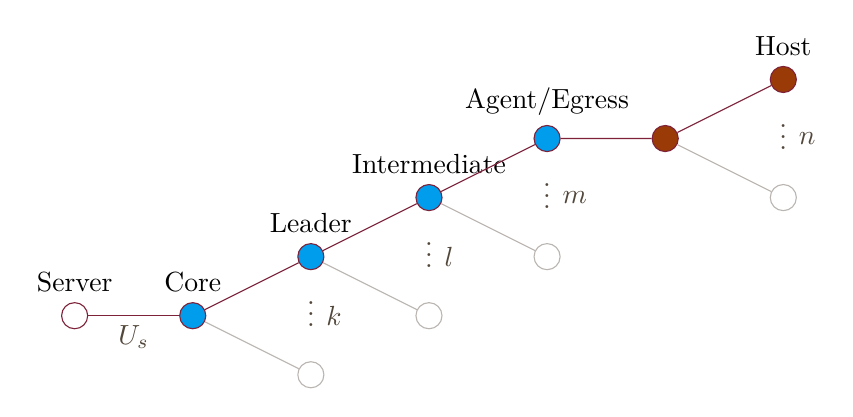
\begin{tikzpicture}[
				texts/.style = {text=black},
				labeltexts/.style = {text=uofgsandstone},
				treeline/.style = {draw=uofgburgundy},
				treenode/.style = {texts, circle, centered, fill=white, treeline},
				load/.style = {fill=uofgcobalt},
				external/.style = {fill=uofgrust},
				hideline/.style = {draw=uofgsandstone!40!white},
				hidenode/.style = {treenode, hideline},
				grow'=right
				]
				\node[treenode, label={[texts]above:Server}] (root) {}
				child [treeline] { node [treenode, load, label={[texts]above:Core}] (sswitch) {}
					child [treeline] { node [treenode, load, label={[texts]above:Leader}] (teaml) {} 
						child [treeline] { node [treenode, load, label={[texts]above:Intermediate}] (inter) {}
							child [treeline] { node [treenode, load, label={[texts]above:Agent/Egress}] (agent) {}
								child [treeline] { node [treenode, external] (extern) {}
									child [treeline] { node [treenode, external, label={[texts]above:Host}] (host) {} }
									child [hideline] { node [hidenode] (endhost) {} }
								}
							}
							child [hideline] { node [hidenode] (endagent) {} }
						}
						child [hideline] { node [hidenode] (endinter) {} }
					}
					child [hideline] { node [hidenode] (endteaml) {} }
					edge from parent
					node[below, labeltexts] {$U_s$}
				};
				
				%\draw[-] (teaml) -- (endteaml);
				\node [labeltexts] (kdots) at ($(teaml)!0.5!(endteaml)$) {$\rvdots$};
				\node [labeltexts, right = -0.1cm of kdots] {$k$};
				\node [labeltexts] (ldots) at ($(inter)!0.5!(endinter)$) {$\rvdots$};
				\node [labeltexts, right = -0.1cm of ldots] {$l$};
				\node [labeltexts] (mdots) at ($(agent)!0.5!(endagent)$) {$\rvdots$};
				\node [labeltexts, right = -0.1cm of mdots] {$m$};
				\node [labeltexts] (ndots) at ($(host)!0.5!(endhost)$) {$\rvdots$};
				\node [labeltexts, right = -0.1cm of ndots] {$n$};
				\end{tikzpicture}
			}
			\caption{
				Network topology diagram.
				Red nodes are external, blue nodes feature in the state vector.
				Any packet drop occurs when forwarding packets from an egress switch to its parent (intermediate) switch.
			}
		\end{figure}
	\end{column}
\end{columns}
\end{frame}

\begin{frame}{The case for finer granularity}
	\begin{columns}
	\begin{column}{0.45\linewidth}
		\begin{itemize}
			\item Learner/host ratio (action/host ratio) affects host QoS.
			
			\item Reduced service guarantees by nature of \emph{pushback} model.
			\begin{itemize}
				\item \alert{Worse with good-faith TCP congestion avoidance}.
			\end{itemize}
			%This is exacerbated by TCP congestion avoidance---legit hosts will be punished far more severely, bad actors don't care!
			
%			\item More granular $\implies$ should focus on flow stats, \alert{not aggregates} like now! %Alongside this higher-granularity view, reformulation to include flow characteristics in the decision-making process.
		\end{itemize}
	\end{column}
	\begin{column}{0.5\linewidth}
		\begin{figure}
			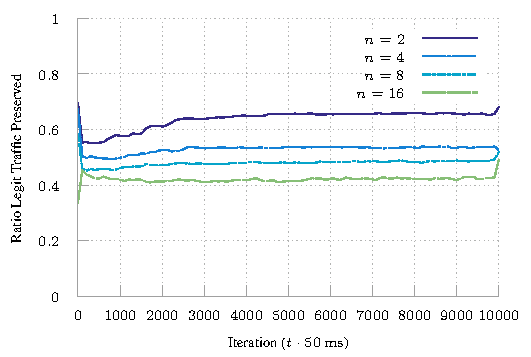
\includegraphics[width=\linewidth]{../plots/online-varyN-binary.pdf}
			\caption{Service quality decreases as actions become less granular (affecting $n$ hosts at once).}
		\end{figure}
	\end{column}
	\end{columns}
\end{frame}

\begin{frame}{The case for finer granularity}
\centering
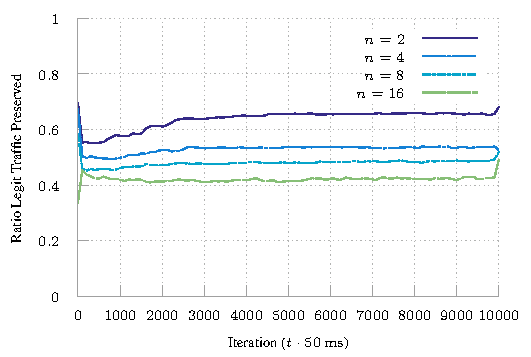
\includegraphics[width=0.8\linewidth]{../plots/online-varyN-binary.pdf}
\end{frame}

\begin{frame}{On collateral damage}
\begin{columns}
	\begin{column}{0.5\linewidth}
		\begin{figure}
			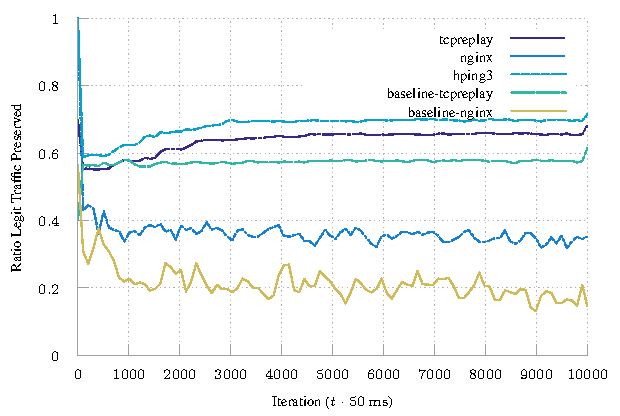
\includegraphics[width=\linewidth]{../plots/online-varyN-nginx.pdf}
			\caption{Explicit UDP traffic matches replayed traces (tcpreplay vs hping3). TCP traffic (nginx) is severely punished.}
		\end{figure}
	\end{column}
	\begin{column}{0.45\linewidth}
		\begin{itemize}
			\item Is the simulation environment of past work complete?
			\item \alert{No.} It's reliant on a numerical simulator, derived from observations of \emph{traces}.
			\item UDP benign traffic similar trend to replayed TCP traces, which matches the original results.
			\item Live TCP responds very badly.
		\end{itemize}
	\end{column}
\end{columns}
\end{frame}

\begin{frame}{On collateral damage}
\centering
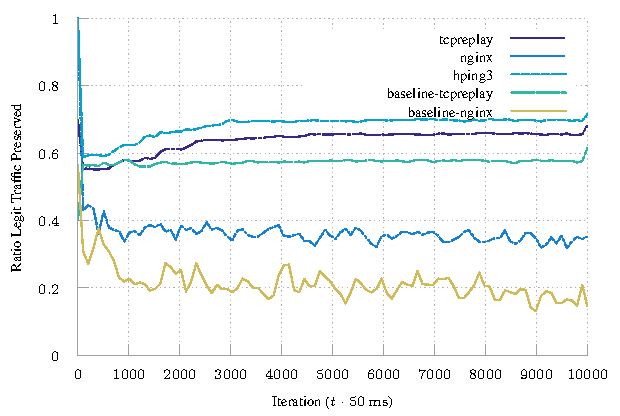
\includegraphics[width=0.8\linewidth]{../plots/online-varyN-nginx.pdf}
\end{frame}

\begin{frame}{And the replication reveals...}	
\begin{itemize}
	\item Network topology has no basis in reality---admitted by its \emph{own} source work \footcite{DBLP:journals/ccr/MahajanBFIPS02a}.
	
	\item Action granularity causes more collateral damage than we'd like...
	
	\item ...and the picture is worse still for legitimate TCP flows.
	
	\item Reward function needs a priori knowledge/reliable estimates to learn online.
	
	\item \alert{But on tbe plus side, action computation is fast: \SIrange{80}{100}{\micro\second}.}
\end{itemize}
\end{frame}

\begin{frame}{How can we use these observations? (The Immediate Future)}
\begin{itemize}
	\item \textbf{\alert{Why not take actions on a per-flow basis}}?
	\begin{itemize}
		\item Solves the granularity issues by construction.
		\item Allows different treatment by flow features (i.e., protocol).
	\end{itemize}
	\item Need to rethink state space: more costly computation, but we have room to work in.
	\begin{itemize}
		\item We need any additions to be justified beyond just ``more data'', since \alert{changes affect training time and execution time}.
	\end{itemize}
	\item How do we select flows to act upon?
\end{itemize}
\end{frame}

\begin{frame}{A candidate state space}
\begin{description}
	\item[Global State] The existing state space.
	\item[Local State] (At least) the following:
	\begin{itemize}
		\item \textbf{Src/dst IP, Port, Protocol}---identification.
		\item \textbf{Flow size, duration, rate}---standard features.
		\item \textbf{\alert{Last action taken}}---encode belief/forgiveness.
		\item \textbf{\alert{Correspondence ratio}}---explicitly capture asymmetry.
		\item \textbf{\alert{$\Delta$rate}}---model how a flow's behaviour changes post-action.
		\item Other features?
	\end{itemize}
\end{description}

And then finding a suitable discretisation...
\end{frame}

\begin{frame}{The Near Future}
\begin{itemize}
	\item Flow selection strategies (guided action calculation).
	\item Reward functions without dependence on ahead-of-time knowledge.
	\begin{itemize}
		\item I.e., for certain distributions of communication we might want to maximise link utilisation in both directions.
	\end{itemize}

\item Deriving normal model behaviour from traces.
\begin{itemize}
	\item We only need to simulate specific behaviour to test these enhancements, but that can become more representative.
\end{itemize}
\end{itemize}
\end{frame}

\begin{frame}{The Far Future}
\begin{itemize}
	\item Other problems.
	\begin{itemize}
		\item New action spaces, careful consideration.
	\end{itemize}
\item Adversarial capabilities---evasion and poisoning attacks.
\item Knowledge-sharing between agents: cost-modelling and optimisation.
\item Test deployments in real networks.
\end{itemize}
\end{frame}

\begin{frame}[standout]{Conclusion}
	We've looked at...
	\begin{itemize}
		\item A quick introduction to RL, and its \alert{importance to future networks} for optimisation and control of certain classes of problem.
		\item A recent `direct control' approach to intrusion prevention, and \alert{its significant weaknesses}.
		\item \alert{Intended improvements} specifically targeting these weaknesses.
	\end{itemize}
	
	\alert{Questions?}
\end{frame}

\appendix

\begin{frame}[allowframebreaks]{References}
\printbibliography[heading=none]
\end{frame}

\end{document}
